\chapter{Alguns exemplos}
\label{cap:exemplos}

% figuras estão no subdiretório "figuras/" dentro deste capítulo
\graphicspath{\currfiledir/figuras/}

%=====================================================

\section{Guias de \LaTeX}

Este modelo contém exemplos para os padrões de inserção de figuras, tabelas, listas de itens, bibliografia, etc. Em caso de dúvidas ou discordância, Pode-se entrar em contato com a direção ou secretaria do programa. Obviamente, críticas (construtivas) e sugestões são muito bem-vindas.

Para aprender a usar \LaTeX, um bom guia introdutório disponível na Internet é \cite{oetiker07}, que também tem uma versão em português. Para tópicos mais avançados consulte \cite{goossens93}.

%=====================================================

\section{Estrutura do texto}

Para melhorar a legibilidade do texto, deve ser evitado o uso de subdivisões mais profundas que a subseção (por exemplo, subsubseções). Se elas forem absolutamente necessarias, não devem ser numeradas. Deve-se analisar a possibilidade de uso de uma lista de itens em seu lugar. O número de níveis de texto do documento não deve exceder três: capítulo, seção e subseção. O uso de mais que três níveis dificulta a leitura e prejudica muito a estética do texto.

%=====================================================

\section{Estilo de redação}

Ao elaborar o texto da dissertação ou da tese, o mais indicado é o uso do verbo na forma impessoal. Exemplos:

\begin{itemize}
\item ... utilizaram-se os seguintes dados ...
\item ... elaborou-se de forma precisa ...
\item ... trata-se os algoritmos ...
\item ... foram obtidos resultados significativos ...
\end{itemize}

Além disso, deve-se a todo custo evitar a ``linguagem de revista'', com expressões como ``sensacional'', ``impressionante'', ``monstruoso'', etc (por exemplo: ``Os resultados obtidos são sensacionais, sobretudo considerando a monstruosa margem de erro.'').

%=====================================================

\section{Alguns exemplos}

Esta seção traz algus exemplos de elementos típicos de um texto científico, como figuras, tabelas e fórmulas matemáticas.

%=====================================================

\subsection{Exemplo de figura}

A forma sugerida para incluir figuras em um documento \LaTeX\ é importá-las usando o pacote \texttt{graphicx}. Como formatos gráficos sugere-se:

\begin{itemize}

\item Formatos \emph{raster}, como PNG (\emph{Portable Network Graphics}) ou JPG (\emph{Joint Photographic Experts Group}) para fotografias; procure usar uma resolução de ao menos 150 dpi (\emph{dots per inch}).

\item Formatos vetoriais, como PDF (\emph{Portable Document Format}) ou EPS (\emph{Extended PostScript}) para diagramas e gráficos\footnote{NUNCA use JPG ou GIF para desenhos vetoriais, pois o resultado final geralmente fica borrado.}.

\end{itemize}

A maior parte das ferramentas permite exportar figuras nesses formatos (a figura do exemplo foi produzida com o \emph{Inkscape}, um programa livre multiplataforma). A figura \ref{fig:comun-intra-inter} mostra um exemplo de inclusão de figura em PDF.

% exemplo de inserção de figura
\begin{figure}[!htb]
\centering
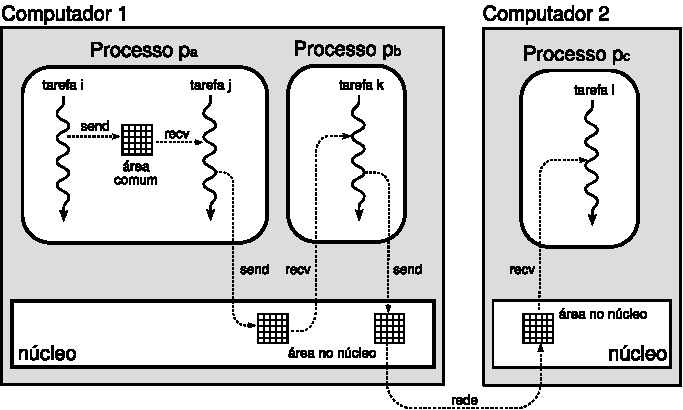
\includegraphics[width=12cm]{exemplo-figura.pdf}
\caption{Comunicação inter-processos.}
\label{fig:comun-intra-inter}
\end{figure}

Para mais informações consulte \cite{goossens93}.

%=====================================================

\subsection{Exemplo de tabela}

Tabelas são elementos importantes de um documento. No \LaTeX\ as tabelas podem ser objetos flutuantes (definidas no ambiente \texttt{table} e referenciadas por números usando \texttt{label} e \texttt{ref}) ou objetos fixos simples, criados pelo ambiente \texttt{tabular}. A tabela \ref{tab:modelos} é um exemplo de tabela flutuante, cuja posição no texto pode variar em função das quebras de página.

\begin{table}[!htp]
\centering
\caption{Os 16 modelos centrais do UCON$_{\mathrm{ABC}}$}
\label{tab:modelos}
\begin{tabular}{|c|cccc|}
\cline{2-5}
\multicolumn{1}{c|}{}& 0 (imutável) & 1 (\emph{pre-update}) & 2 (\emph{on-update}) & 3 (\emph{pos-update}) \\
\hline
\texttt{preA} & \textbullet & \textbullet & -- & \textbullet \\
\hline
\texttt{onA} & \textbullet & \textbullet & \textbullet & \textbullet \\
\hline
\texttt{preB} & \textbullet & \textbullet & -- & \textbullet \\
\hline
\texttt{onB} & \textbullet & \textbullet & \textbullet & \textbullet \\
\hline
\texttt{preC} & \textbullet & -- & -- & -- \\
\hline
\texttt{onC} & \textbullet & -- & -- & -- \\
\hline
\end{tabular}
\end{table}

%=====================================================

\subsection{Exemplo de fórmula}

Equações destacadas devem ser numeradas como mostra a equação \ref{eq:relatividade}:

\begin{equation}
E = m \times c^2
\label{eq:relatividade}
\end{equation}

%=====================================================

\subsection{Exemplos de código-fonte}

Códigos-fonte podem ser produzidos de forma simples através do ambiente \texttt{verbatim}, como mostra este exemplo:

\begin{footnotesize}
\begin{verbatim}
#include <stdio.h>

int main (int argc, char *argv[])
{
   int i ;                           // uma variavel local

   for (i=0; i< 100; i++)            // um laço for
      printf ("i vale %d\n", i) ;    // uma saída na tela
}
\end{verbatim}
\end{footnotesize}

No entanto, é preferível usar pacotes especializados para a edição ou inclusão de códigos-fonte, como o pacote \texttt{listings}. Eis um exemplo de código-fonte escrito com esse pacote:

% exemplo de código-fonte definido no próprio texto

\begin{lstlisting}
#include <stdio.h>

int main (int argc, char *argv[])
{
   int i ;                           // uma variável local

   for (i=0; i< 100; i++)            // um laço for
      printf ("i vale %d\n", i) ;    // uma saída na tela
}
\end{lstlisting}

Esse pacote também permite incluir códigos-fonte de arquivos externos. Eis um exemplo:

% exemplo de código-fonte incluso

\lstinputlisting{2-fundam/exemplo.c}

%=====================================================

\subsection{Exemplo de algoritmo}

Os pacotes \texttt{algorithm} e \texttt{algorithmic} permitem formatar algoritmos facilmente. Eis um exemplo:

\begin{algorithm}[H]
\caption{Ações de $s_i$ ao encerrar um ciclo:}
\label{alg:on-period-ending}
\begin{small}
\begin{algorithmic}[1]
\FORALL{$x \in \mathcal{K}_i$}
  \STATE{$\mathit{banned}_i(x) \gets$ FALSE}
  \STATE{$mi_i(x) \gets 0$}
  \STATE{$mm_i(x) \gets 0$}
  \STATE{$\mathit{age}_i(x) \gets \mathit{age}_i(x) + 1$}
  \IF{$\mathit{age}_i(x) = \mathit{age}_\mathit{max}$}
     \STATE{$\mathcal{K}_i \gets \mathcal{K}_i - \{x\}$}
     \COMMENT{``esquece'' do servidor $x$}
     \STATE{remove as informações locais sobre $x$}
     \STATE{envia $\mathit{notify}(x,\mathit{undef})$ ao grupo de confiança $\mathcal{T}_i$}
  \ENDIF
\ENDFOR
\end{algorithmic}
\end{small}
\end{algorithm}
 
%=====================================================

\subsection{Exemplo de citação}

Como afirmou Maquiavel em seu livro \emph{O Príncipe}:

\begin{quote}
``Nada é mais difícil de instituir, mais perigoso de conduzir, mais incerto no seu sucesso, do que liderar a introdução de uma nova ordem de coisas... O inovador faz inimigos em todos aqueles que prosperavam sobre as antigas regras, e somente tíbio suporte é esperado daqueles que prosperariam na novidade, porque os homens são geralmente incrédulos, nunca realmente confiam nas coisas novas, a menos que as tenham testado em experiência''.
\end{quote}

%=====================================================

\section{Uma seção}

\subsection{Uma subseção}

\subsubsection{Uma subsubseção}

%=====================================================

\section{Conclusão}

Todo capítulo (com exceção da introdução e da conclusão) deve encerrar com uma pequena conclusão local, resumindo os tópicos apresentados no capítulo e preparando o leitor para o próximo capítulo (exceto se esse for a conclusão geral). Caso o capítulo tenha apresentado resultados obtidos pelo próprio autor, estes devem ser sucintamente relembrados aqui.

%=====================================================
